%%% fig:taxonomic_profiler
\begin{figure}[hbt]
    \centering
    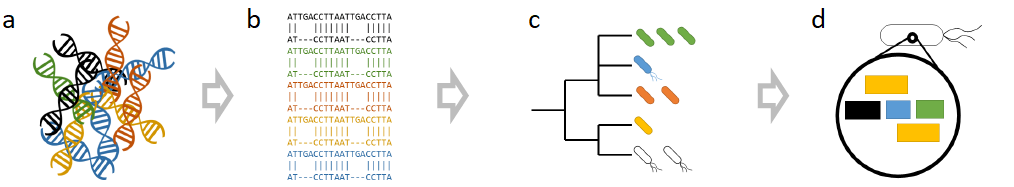
\includegraphics[width=.8\linewidth]{fig/taxonomic_profiler.png}
    \caption{
        (a) Raw reads from the sequencing machine are demultiplexed into individual samples. Then, each read is quality controlled with by removing adapters, low quality bases and contaminates such as host reads \cite{consortium_structure_2012}. Optionally, the read pairs can be stitched \cite{magoc_flash:_2011}. (b) The quality-controlled reads are aligned against a database of known genomes to identify each read's most likely source taxon \cite{langmead_fast_2012}. (c) The taxa that are hit are filtered out and summarized at a specific level. These processing steps include last common ancestor assignment \cite{hong_pathoscope_2014}, genome coverage analysis \cite{wood_kraken:_2014}, and redistribution of reads to a specific taxonomic level \cite{lu_bracken:_2017}. (d) After the taxonomic prediction is set, the full functional repertoire of genes is directly observed through a bag-of-genes approach or predicted through a per microbe approach \cite{langille_predictive_2013}.
    }
    \label{fig:taxonomic_profiler}
\end{figure}

%%% fig:shogun_schematic
\begin{figure}[hbt]
    \centering
    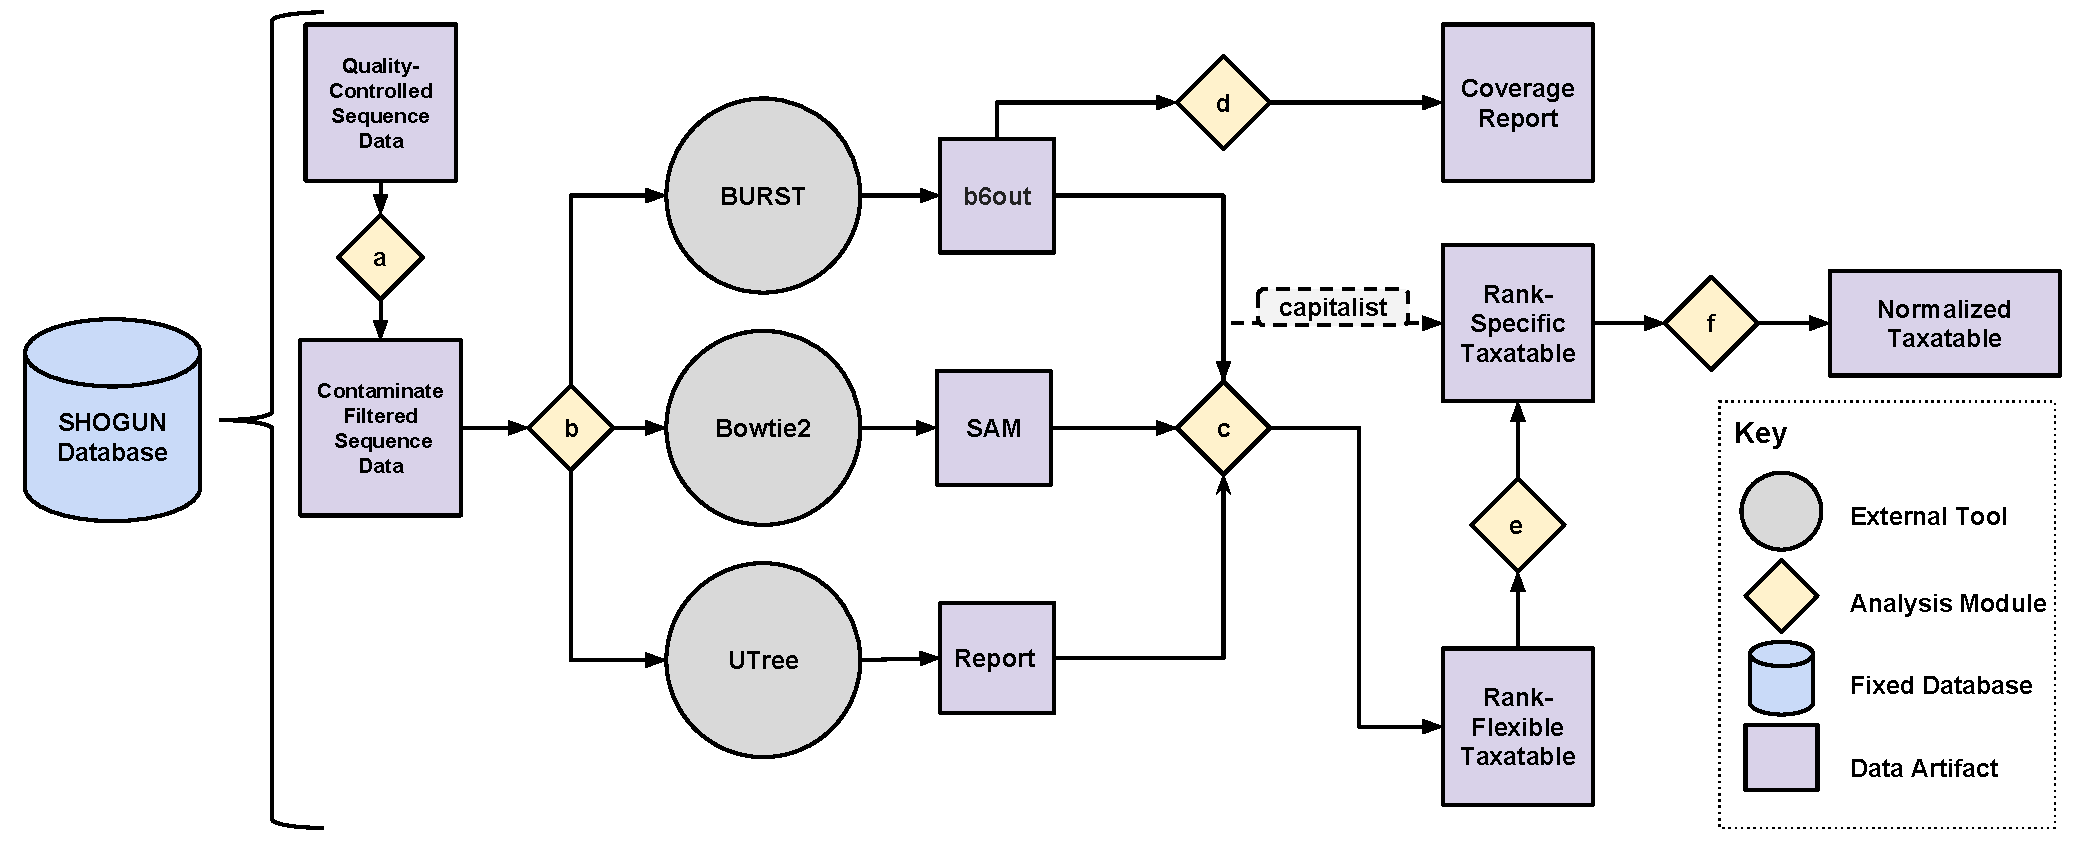
\includegraphics[width=0.8\linewidth]{fig/shogun_schematic.pdf}
    \caption{
        Schematic overview of the shallow-shotgun computational pipeline SHOGUN. For every step in the SHOGUN pipeline, the user must supply the pre-formatted SHOGUN database folder. To run every step shown here in a single command, the user can select the \code{pipeline} subcommand. Otherwise, the analysis modules can be run independently. (a) \code{filter} - The input quality-controlled reads are aligned against the contaminate database using BURST to filter out all reads that hit human associated genome content. (b) \code{align} - The input contaminate filtered reads are aligned against the reference database. The user has the option to select one or all of the three alignment tools BURST, Bowtie2, or UTree. (c) \code{assign\_taxonomy} - Given the data artifacts from a SHOGUN alignment tool, output a Biological Observation Matrix (BIOM) \cite{mcdonald_biological_2012} format taxatable with the rows being rank-flexible taxonomies, the columns are samples, and the entries are counts for each given taxonomy per sample. The alignment tool BURST has two run modes, taxonomy and capitalist. If the capitalist mode is enabled, a rank-specific BIOM file is output instead. (d) \code{coverage} - The output from BURST can be utilized to analyze the coverage of each taxonomy across all samples in your alignment file. This can useful for reducing the number of false positive taxonomies. (e) \code{redistribute} - The rank-flexible taxatable is summarized into a rank-specific taxatable. This summarizes both up and down the taxonomic tree. (f) \code{normalize} - Each sample in the taxatable is normalized to the median depth of all the samples.
    }
    \label{fig:shogun_schematic}
\end{figure}

%%% fig:hmp_beta
\begin{figure}[hbt]
    \centering
    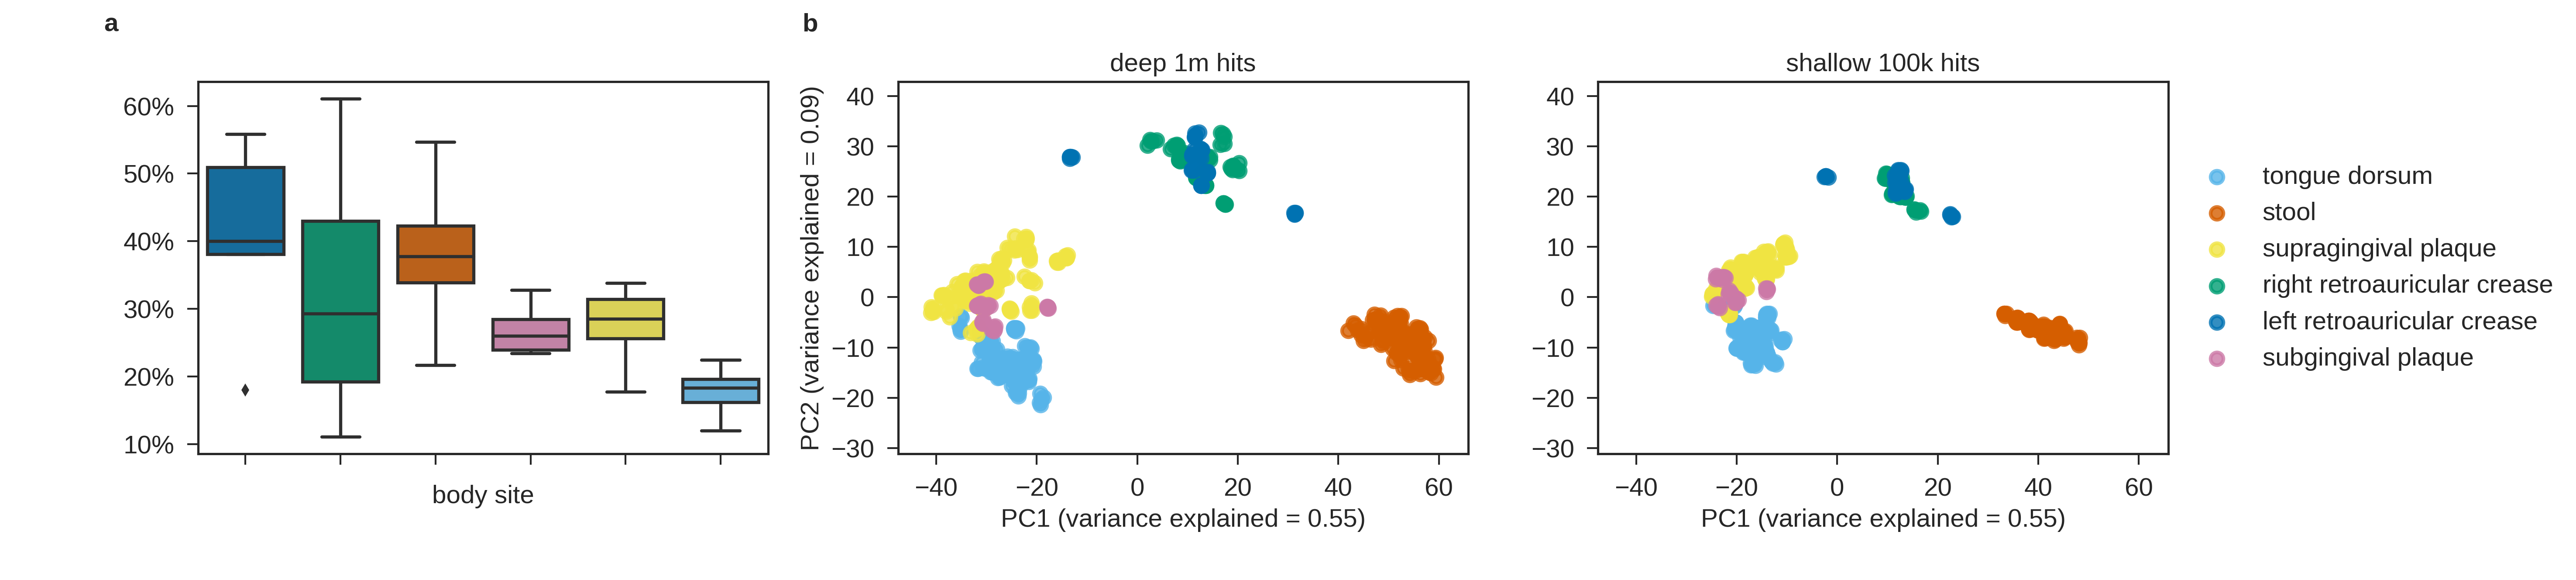
\includegraphics[width=0.8\linewidth]{fig/hmp_beta.png}
    \caption{
        (a) The alignment rate of the sequences to the reference database per body site using BURST capitalist. Most samples aligned at approximately a 25\% rate at 98\% sequence identity to a genome in the reference database. (b) Beta-diversity plots using Euclidean distance on Centered Log-Ratio (CLR) with multiplicate-replacement transformed data. Shown here are the two dimensions that explain the most variance in the data after Principal Components Analysis (PCA). Notice that the groups clearly separate by body sites at both deep- (ADONIS p-value .008**, beta-dispersion p-value=.003**) and shallow-sequencing depths (ADONIS p-value=.02*, beta-dispersion p-value=.01*). 
    }
    \label{fig:hmp_beta}
\end{figure}

%%% fig:hmp_alpha
\begin{figure}[hbt]
    \centering
    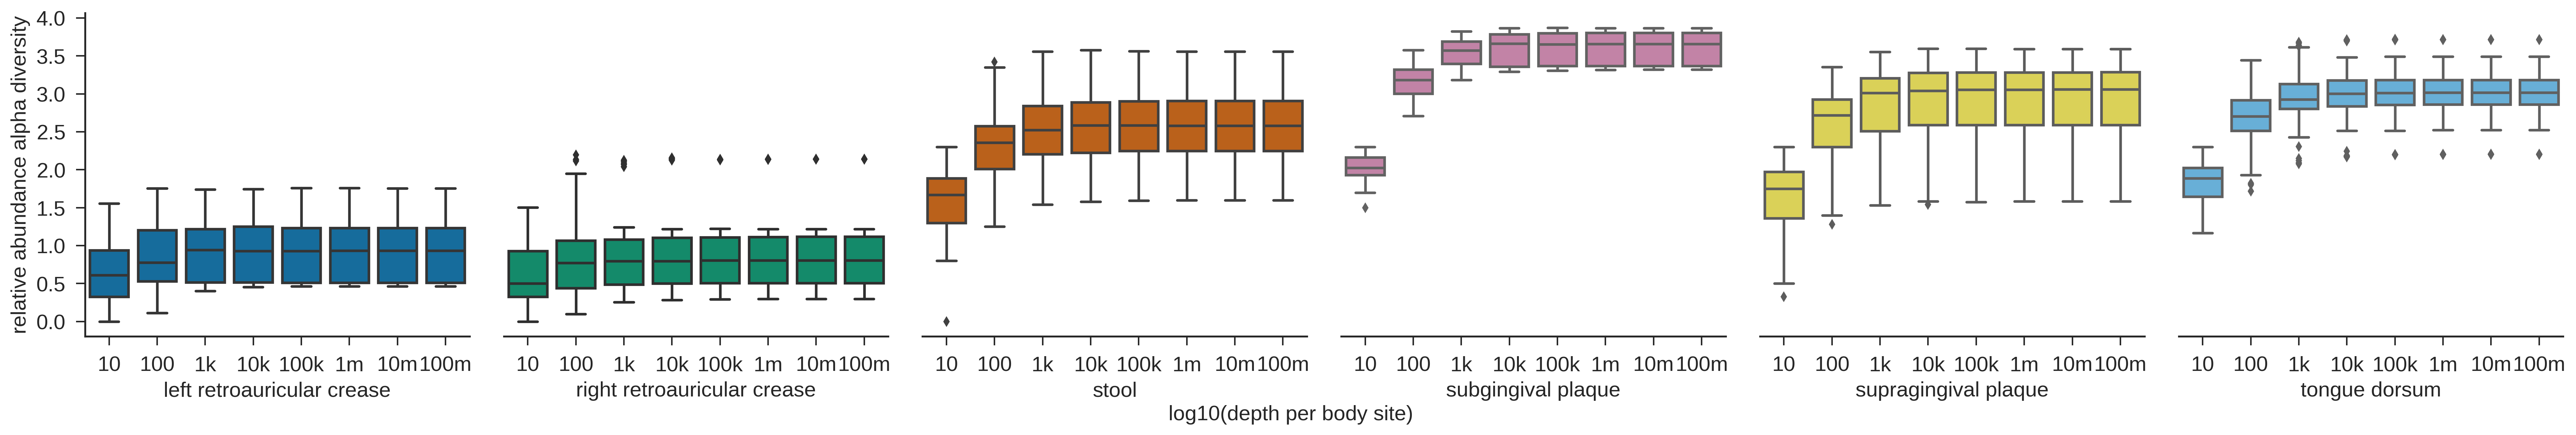
\includegraphics[width=0.8\linewidth]{fig/hmp_alpha.png}
    \caption{
        The alpha-diversity using Shannon index at different bootstrapped depths per body site. Each count vector is summarized using a relative abundance transformation. In all cases, full alpha-diversity is captured between a thousand and ten-thousand counts per sample.
     }
     \label{fig:hmp_alpha}
\end{figure}

%%% fig:hmp_taxa
\begin{figure}[hbt]
    \centering
    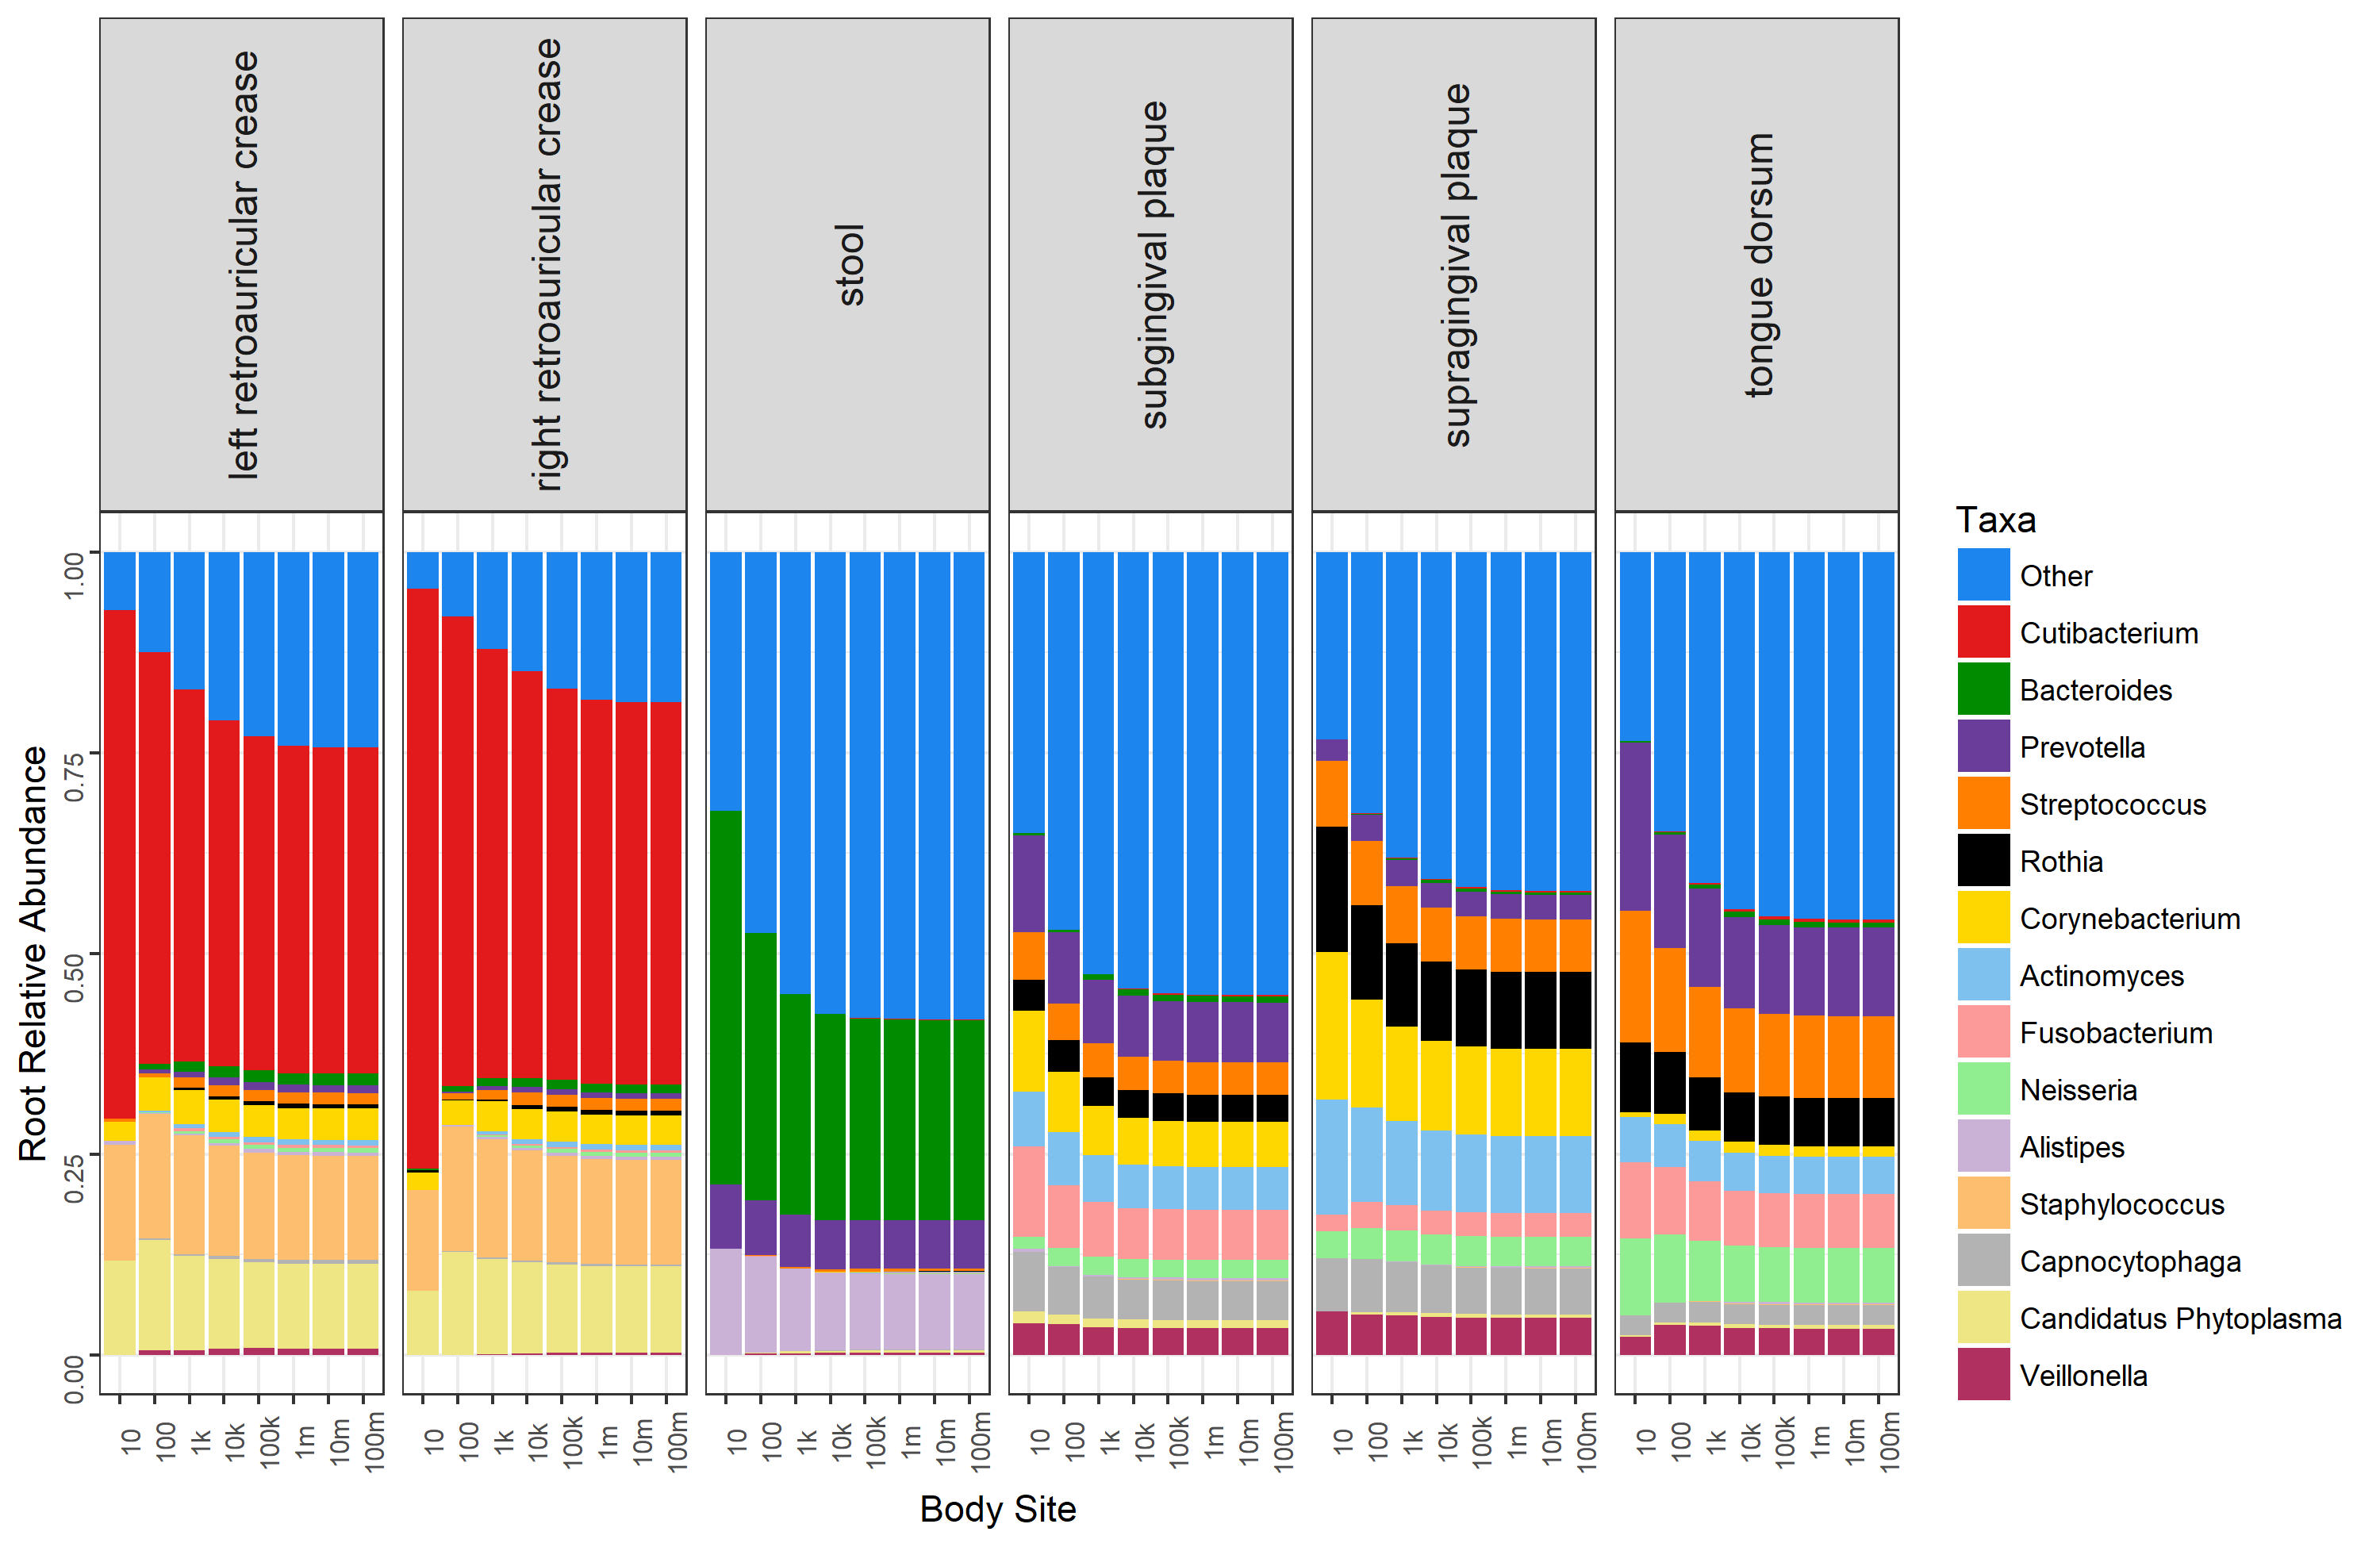
\includegraphics[width=0.99\linewidth]{fig/hmp_taxa.png}
    \caption{
        Taxa-summary plots at genus-level (for visualization convenience) stratified by body site by increasing depth. Visually depicted is the transition of the relative abundance vectors to the stabilized full depth relative abundance between a thousand and ten-thousand counts per sample.
    }
    \label{fig:hmp_taxa}
\end{figure}

%%% fig:karlsson2013_f1_combined
\begin{figure}[hbt]
    \centering
    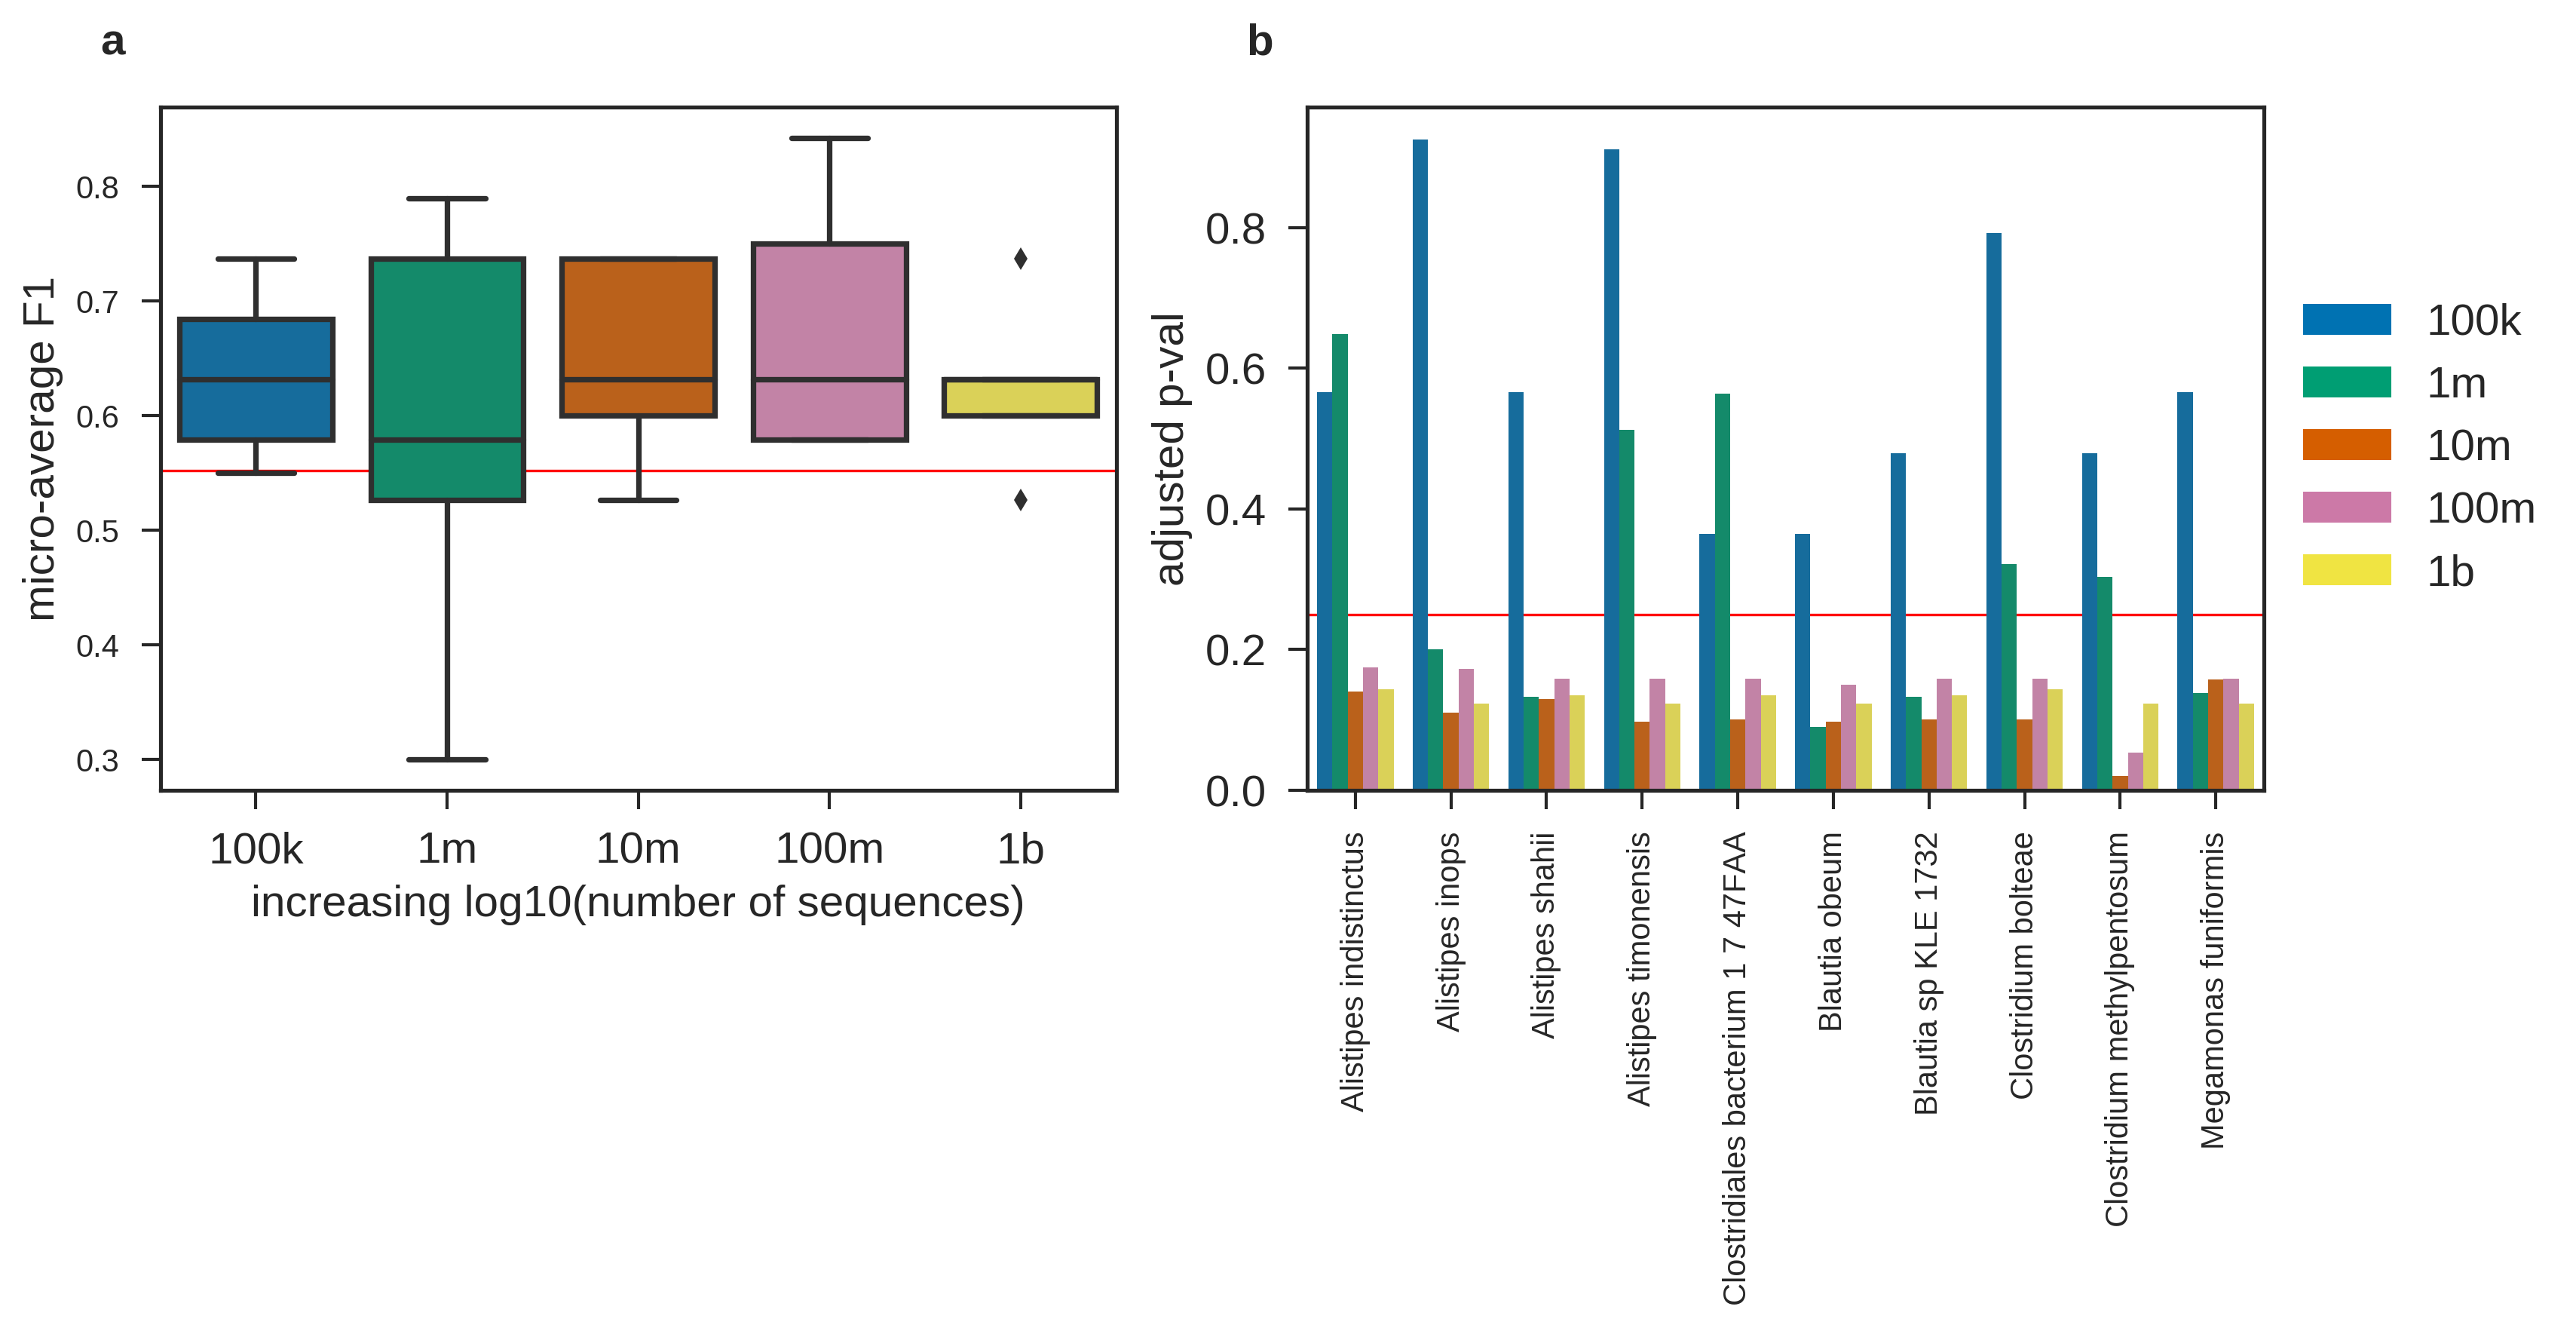
\includegraphics[width=0.8\linewidth]{fig/karlsson2013_f1_combined.png}
    \caption{
        (a) The micro-averaged F1-Score from 10-fold cross-validation on predicting normal glucose tolerance (NGT) versus type-2 diabetes (T2D) on centered log-ration (CLR) multiplicative replacement transformed Karlsson dataset. The classifier used was a Support Vector Machine (SVM) with a linear kernel. The red line is the baseline classifier that predicts majority class (NGT samples = 43, T2D samples = 53). At all subsampled depths, the classifier is able to outperform the baseline classifier verifying the discriminative correlation of microbes with T2D. (b) The Benjamini-Hochberg adjusted Wilcoxon signed-rank p-values for the differentially abundant species between T2D and NGT at varying depths. Displayed are the top ten most differentially abundant species at full depth. The red line is a false-positive rate of 25\%. All species remain significant until a subsampled depth of a thousendth of the original sequences.
    }
    \label{fig:karlsson2013_f1_combined}
\end{figure}

%%% fig:simulations
\begin{figure}[hbt]
    \centering
    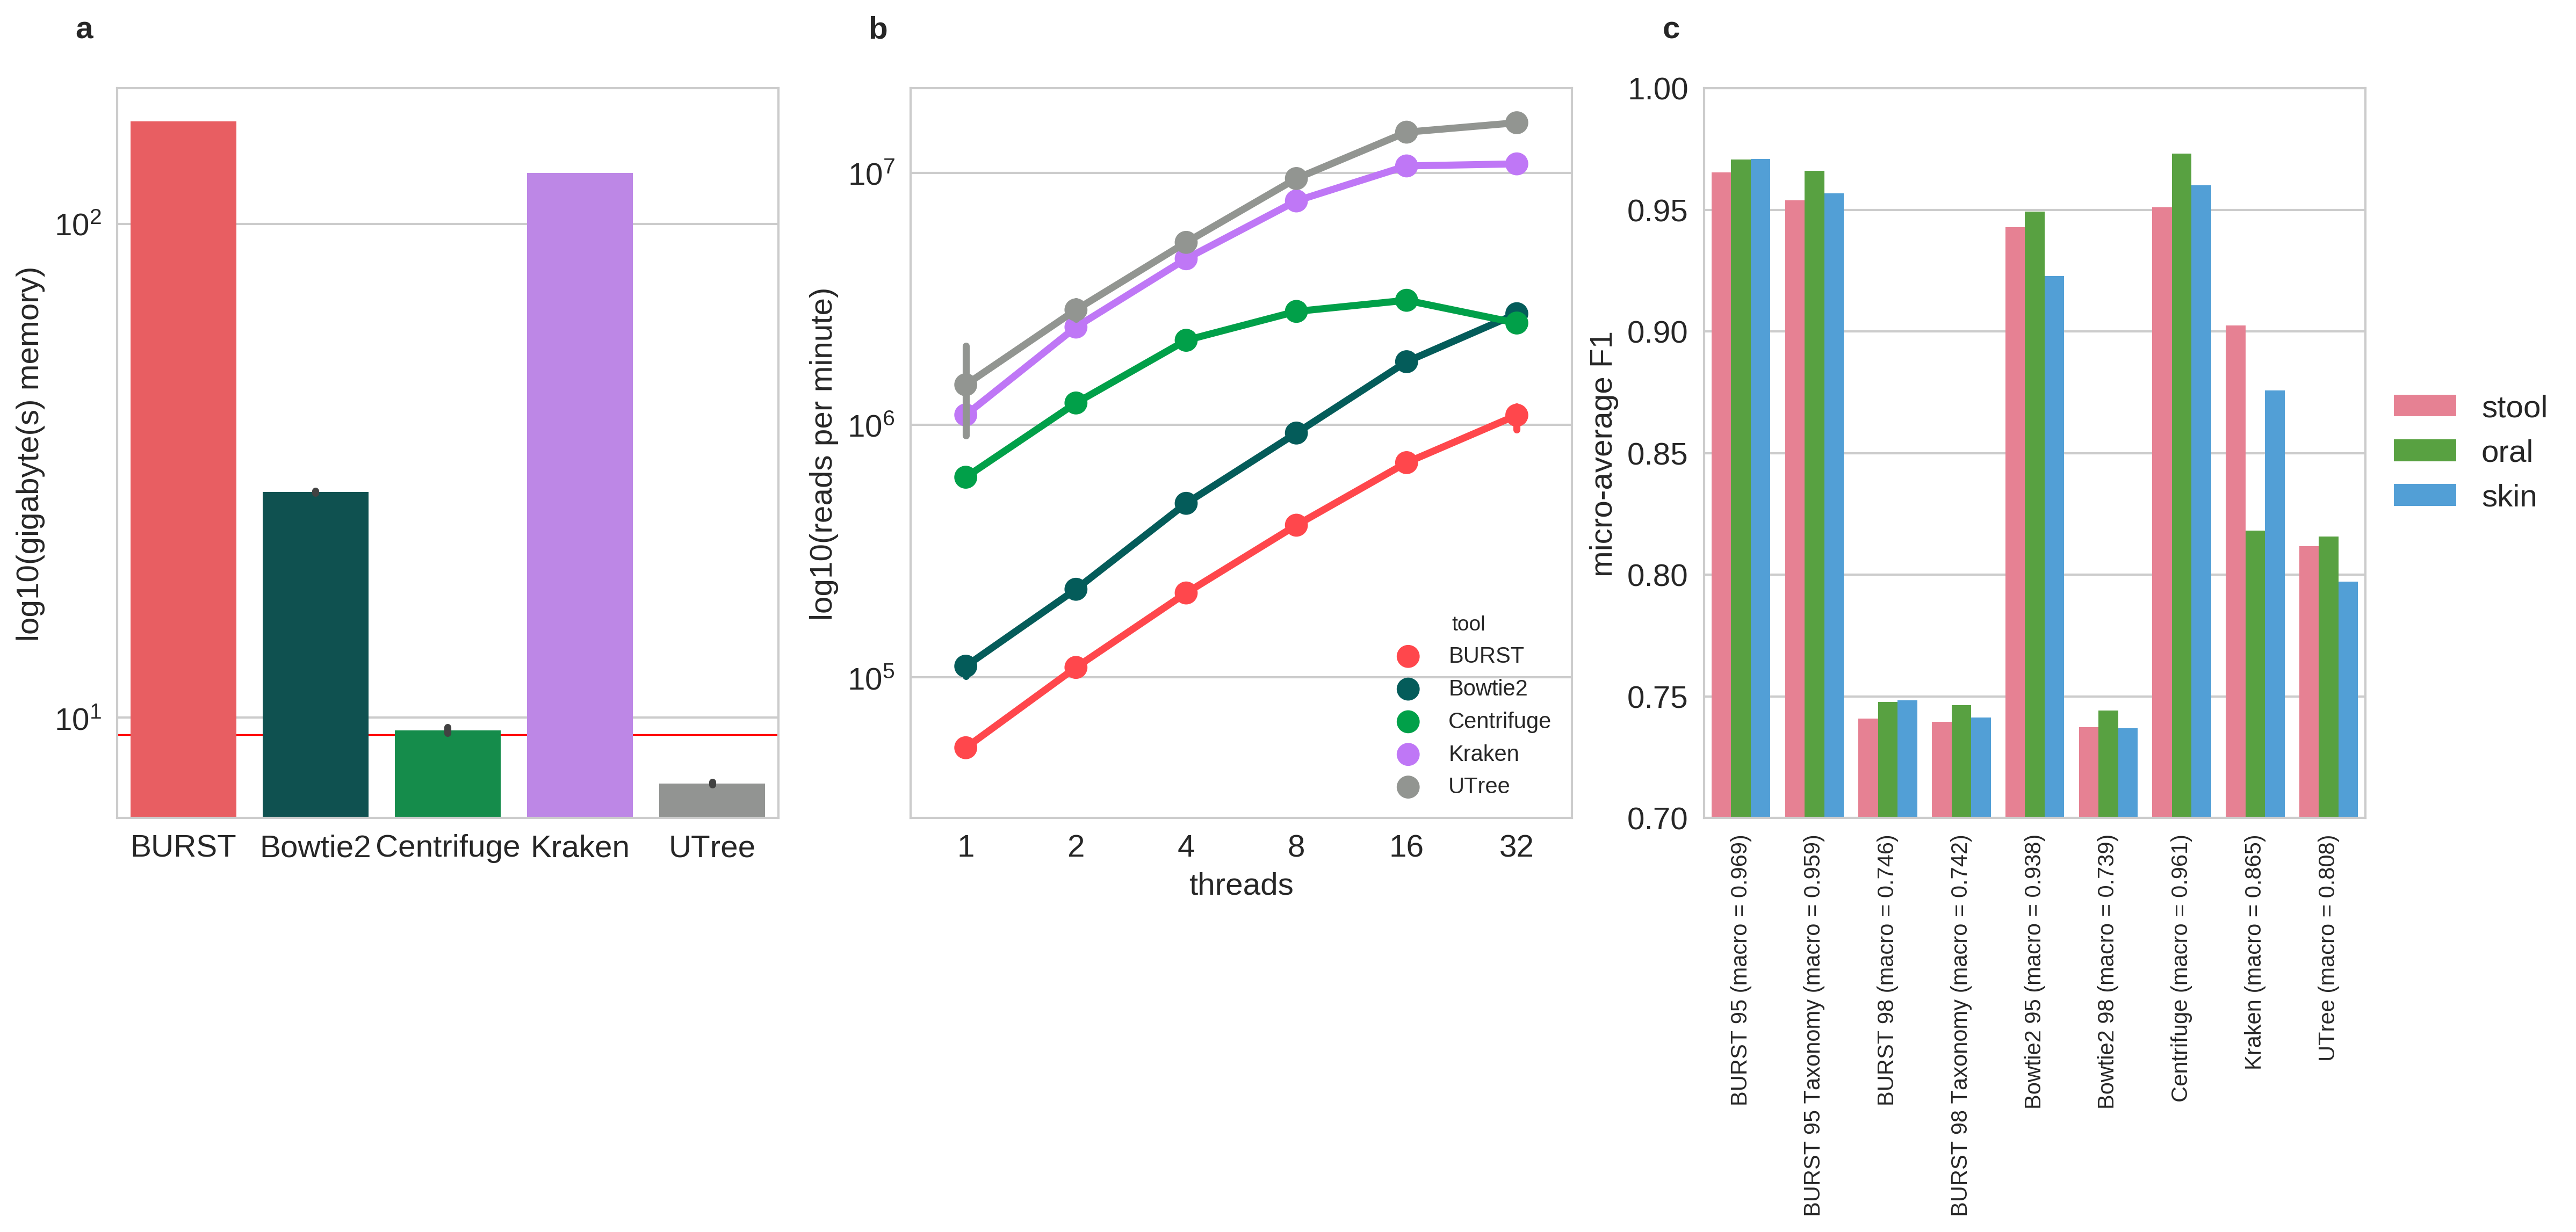
\includegraphics[width=0.8\linewidth]{fig/simulations.png}
    \caption{
        (a) The maximum resident size set (RSS) in Gigabytes of each of the aligners with the Kraken timing dataset. The horizontal red line depicts the size of the original Rep82 database. (b) The scaling and efficiency in reads per minute of each of the aligners across many threads per process. The fastest tools are the alignment free methods Kraken and UTree. Each of the tools scale efficiently across many threads per process. (c) The micro-averaged F1-score of each of the aligners on per read bases on the simulated stool, oral, and skin communities. For the alignment methods, two different thresholds at 95\% and 98\% for alignment identification were set to account for recall bias in highly-divergent reads.
    }
    \label{fig:simulations}
\end{figure}

%%% fig:simulations_js
\begin{figure}[hbt]
    \centering
    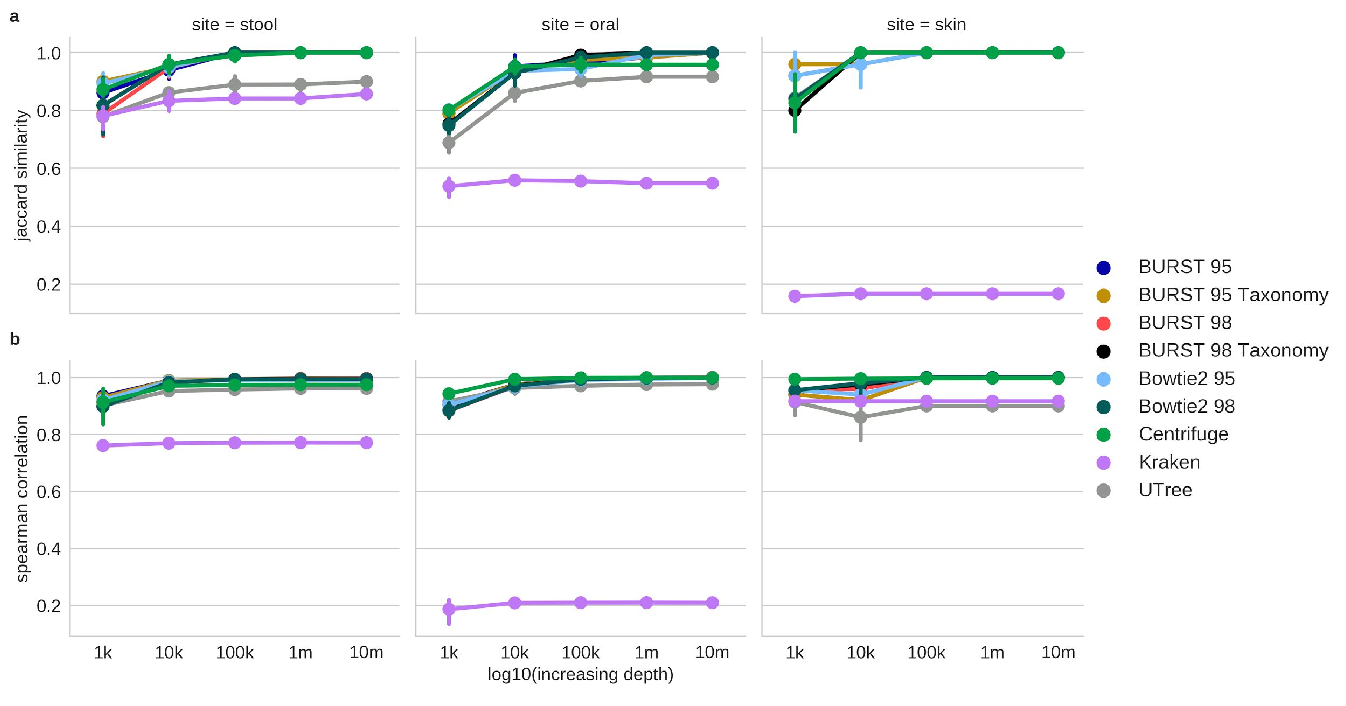
\includegraphics[width=0.8\linewidth]{fig/simulations_js.pdf}
    \caption{
          (a) Rarefaction curves of Jaccard similarity of known species and predicted species for each of the alignment tools on the simulated stool, oral, and skin communities. For most tools, all species are identified between ten-thousand and a hundred thousand reads. (b) The rarefaction curves of Spearman correlation of the tools predicted community with the known community for the simulated dataset. This shows that not only are the correct species identified, but they are also in the correct abundances. 
    }
    \label{fig:simulations_js}
\end{figure}

%%% tab:database_stats
\begin{table}[hbt]
  \centering
  \begin{tabular}{l|r|r}
      \textit{Kingdom} & \textit{Number of Genomes} & \textit{Megabase pairs (Mbp)} \\ \hline
      Archaea & 238 & 627,101.26\\ \hline
      Bacteria & 4,884 & 19,308,087.26\\ \hline
      Plasmid & 614 & 198,476.94\\ \hline
      Viroids & 46 & 15.50\\ \hline
      Viruses & 7,194 & 253,668.36\\ \hline \hline
      \textbf{Total} & \textbf{12,976} & \textbf{20,387,349.32}\\ 
  \end{tabular}
  \caption{
        The number of strains and megabase pairs for each kingdom for all representative Archaea, Bacteria, Plasmid, Viroids and Virus sequences in RefSeq version 82 (Rep82). Each entry in the database is assigned a unique taxonomic string identifier at each level in the taxonomic tree down to strain. An example taxonomic annotation for humans is \code{k\_\_Eukaryota;p\_\_Chordata;c\_\_Mammalia;o\_\_Primates;f\_\_Hominidae;g\_\_Homo;s\_\_Homo\_sapiens;t\_\_}. Each strain is a given a unique entry so that BURST capitalist properly disambiguates reads that hit multiple strains for proper taxonomic profiling and coverage analysis. 
  }
  \label{tab:database_stats}
\end{table}

% Table generated by Excel2LaTeX
%%% tab:discussion
\begin{table}[htbp]
      \centering
      \begin{tabular}{rrll}
      \multicolumn{1}{l}{\textit{Approach}} & \multicolumn{1}{l}{\textit{Examples}} & \textit{Pros} & \textit{Cons} \\
      \midrule
      \midrule
      \multicolumn{1}{l}{\textbf{Last Common Ancestor Alignment}} & \multicolumn{1}{l}{Bowtie2 Taxonomy} & Highest Precision & High RAM \\
            & \multicolumn{1}{l}{BURST Taxonomy} &       & \multicolumn{1}{p{9.5em}}{Slow} \\
            &       &       & No coverage analysis \\
      \midrule
      \multicolumn{1}{l}{\textbf{Exhaustive Alignment}} & \multicolumn{1}{l}{BURST Capitalist} & Highest F1 Accuracy & High RAM \\
            &       & Highest Recall & Slow \\
      \midrule
      \multicolumn{1}{l}{\textbf{Marker Gene}$^\dagger$} & \multicolumn{1}{l}{Metaphlan} & Low RAM & Sparse Database \\
            &       & Fast  &  \\
      \midrule
      \multicolumn{1}{l}{\textbf{Exact K-mers}} &       & Fastest & No coverage analysis \\
            &       &       & Sensitive to indels \\
      \cdashlinelr{2-4}
            & \multicolumn{1}{l}{Kraken} &       & High RAM \\
            &       &       & Large Database \\
      \cdashlinelr{2-4}
            & \multicolumn{1}{l}{Utree} & Lowest RAM &  \\
            &       & Smallest Database &  \\
      \midrule
      \multicolumn{1}{l}{\textbf{Longest Common Substring}} & \multicolumn{1}{l}{Centrifuge} & Fast  & No coverage analysis \\
            &       & Low RAM & Sensitive to indels \\
      \bottomrule
      \multicolumn{4}{l}{$^\dagger$\footnotesize{ Marker gene taxonomic profilers were not evaluated in this study due to complexity of creating a database and low alignment rates.}}
      \end{tabular}%
      \caption{
            Summarization of the many tools tested in this paper for shallow-shotgun sequencing. While this list is not comprehensive, we recommend using any tools in the approaches listed as legitimate options for analysis of shallow-shotgun data except for a marker gene$^\dagger$ approach. From the tools surveyed, we found that BURST capitalist returns the most accurate results if properly tuned at the cost of high RAM usage and compute time. If computer resources is a concern, we recommend using either UTree on a computer with over 8GB RAM or Centrifuge on a computer with over 16GB RAM.
      }
      \label{tab:discussion}
\end{table}
